\subsection{Bayesian Optimization}
In general, the goal of any optimization is to find the global (or a local) minimum/maximum of some function $f(x)$ on some input set $\mathcal{X}$. In our case, this function is identified with our classifier, whereas $x$ can be interpreted as a point in the corresponding hyperparameter space, and $f(x)$ is the measured accuracy of our classifier for this particular set of hyperparameters. Since this function cannot be expressed with an explicit formula, analytical methods for calculating extrema cannot be applied. Numerical methods which require a lot of iteration before convergence are also problematic, since calculating $f(x)$ is computationally expensive. \par
Bayesian Optimization tries to find the maximum of $f$ by constructing a probabilistic model of this function, which is updated and enhanced in every iteration. Basis for this model is a Gaussian Process. Stochastic processes in general are defined as a (infinite) set of random variables which can be indexed (by time or some underlying space; in our case, this is the hyperparameter space). A stochastic process is now called Gaussian, if any finite collection of those random variables has a multivariate normal distribution, i.e. every finite linear combination of random variables from this process is normally distributed. \par
Given a set of observations $\{x_i,y_i\}$ which are found by testing the classifier with some sets $\{x_i\}$ of hyperparameters, the probalistic model together with these observations induce a so-called \emph{acquisition function} (also known as \emph{utility function}) $a: \mathcal{X} \rightarrow \mathbb{R}^+$ , which then is used to calculate the next point $x_{\text{next}} \in \mathcal{X}$ which will be evaluated. \cite{snoek2012practical}

\begin{figure}[H]
	\begin{center}
		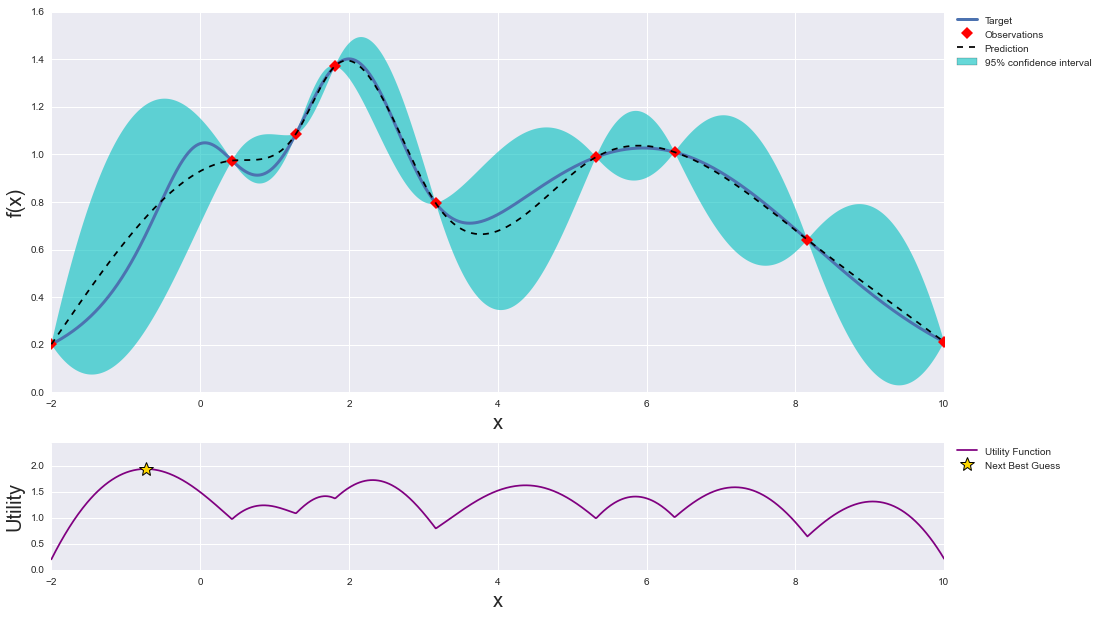
\includegraphics[width=\textwidth]{images/bayesian_optimization_example.png}
		\caption{Toy-example with one-dimensional $f(x)$. The target function also is displayed. Taken from the official Github implementation for Bayesian Optimization. Source: \href{https://github.com/fmfn/BayesianOptimization}{github.com/fmfn/BayesianOptimization}}
		\label{abb:bayes_opt_example}
	\end{center}		
\end{figure}
In our implementation, Bayesian Optimization is used in the One-vs-Rest-Classifier to optimize the hyperparameters of each individual internal classifier. 